\chapter{Multimodal Contextual Video Annotation}
\minitoc
%\cleardoublepage

\section{Introduction}
The audio-visual indexing process becomes decisive in order to understand these content easily. Video content annotation is considered as a keystone for the effectiveness of indexing task. Indeed,  different annotation systems and approaches are proposed in litterature.
Earlier approaches like \textit{VideoAnnEx} \cite{Schroeter2004} and \textit{Advene}
\cite{Aubert2005} are simple and non collaborative annotation. The latter has introduced in 2005 (EVA \cite{Volkmer2005} and TRECVID \cite{Ayache2007}). Recently, the relevance feedback has been used to deal with conflicting situations, and then to improve annotation results \cite{Ksibi2011}. However, all the systems above handle concepts only at a semantic level. In this context, we propose a new collaborative annotation approach with a higher semantic
level: the context. The context is important not only in the refinement of annotation results, but also in giving support
to the user when annotating. The annotation process finally provides semantic graphs whose goal is to improve the indexing process \cite{Elleuch2011,Koetters2009,Jiang2009b}. 


\section{The proposed Multimodal Contextual Video Annotation approach}

The proposed Multimodal Contextual Video Annotation approach focus on improving the video annotation results, basically, by the use of contextual information. At first, we handle collaborative annotation and particularly on how to share the previous annotations in order to manage conflict situations. Then, the use of \textit{context} in the annotation process provides answers to the main problem : the same concept can appear differently within different contexts. 

The annotation process consists I  the following components : conceptual/contextual spaces, collaborative annotation, conceptual relationships and finally, the visualization. In what follows, we detail each of these components.

\subsection{Conceptual/Contextual space}
We used LSCOM hierarchical structure to cover the concept space. We used 130 concepts defined in TRECVID 2010 \cite{phd::Oomen2013}.

The contextual space covers informations that could enhance the semantic concept interpretation. Based on the LSCOM ontology, we carried out a study in order to define the contexts to be employed when annotating video shots. A concept is considered as a context if it indicates a spatial or temporal information or en event \cite{Brilhault2009}.

As an example, the concept airplane-flying is considered as a context, since it indicates in its name an event. It complements the semantics of concept airplane by specifying the actual position of this latter.

\subsection{Collaborative annotation}
The collaborative annotation is incorporated in our system in order to attenuate the problem of manual annotation. In fact, annotation systems (like in \cite{Ayache2007}  and \cite{Volkmer2005}) do not allow sharing of previous annotations. Collaboration aspect are integrated in our annotation system. Indeed, a video shot will be annotated be several annotators (or experts). Thus, we defined these tools:

\subsubsection{Detection shots of key frames}
The shot detection component adds useful information for annotating photos and to better identifying the context in which an object appeared : by listening to the sound track or by following the movement of an object.

	\subsubsection{Sharing previous interpretations by other users}
This functionality is very important to manage conflicts
which can appear. For example, for a given image, he can
refer to the previous annotations presented in chronological
order in order to take an idea and to annotate the image correctly. For this feature, we do not manage conflicts \cite{Ksibi2011} by
estimating inter-annotator agreement.
	\subsubsection{Visual Concept suggestion}
When the annotator identifies one concept in an image, the
system can suggests to him some other concepts related
to the chosen one. Also, the system draw a small graph
which present the relationships between the concepts detected in previous annotations. These functionalities are derived from an advanced study on the basis of previous participations of our team in TrecVID, which allowed us to study more closely the relationships between the concepts \cite{Elleuch2011}.
	\subsubsection{Annotation controlled by ontology}

Annotation systems always use an informal annotation (either binary or free texts) (\cite{Volkmer2005} and \cite{Ayache2007}). We propose to
use an annotation which is controlled by using concepts of
L SCOM ontology in order to have a formal and standard annotation. The ontology used in our system is presented by a
tree structure of concepts/contexts. Indeed, this representation allows the annotator to traverse it quickly and to select
the concepts which seem relevant to him.

\subsection{Conceptual relationships}
	\subsubsection{Judgments modeling}
If the image is completely annotated, our system deals with
the annotators judgments by initially applying the majority vote to the context. Indeed, when the majority of the
annotators agree on a context, this latter will be valid for
this image. In the second place, our system calculates the
annotation frequency of each concept and awards them to
the image in order to build, thereafter, the weight vectors of
each concept.

an image is described by different annotators. The system generates then a final annotation for the
latter by applying the standards mentioned earlier. Thus,
we see that all three annotators shall agree on the context
of the image \textit{Outdoor} and on the concepts \textit{Vegetation} and
\textit{Weather}, but one of these three reported the existence of
concepts \textit{Sky} and \textit{Trees}.
	\subsubsection{Extracting conceptual relationships}

To determine the conceptual relationships between the concepts detected during the annotation process, we chose to
represent them in the first place by characteristic vectors. In
the second place, we calculate the inter-concepts similarity
through these representations.

These vectors are built by exploiting the final results of
the process of video annotation. Thus, we define a dimen
sional and dynamic matrix whose lines represent the key
frames annotated and the columns the detected concepts.
As soon as an image is completely annotated, a new line
is added to this matrix. The same thing applies for the concepts: if there is a new detected concept which does not
appear in the matrix, we add a column which presents this
concept.

If the concept is present in the key frame, we give it its
value mentioned in the final results. If not, we give it a
zero This matrix is used to determine, thereafter, the weight
vectors of each concept.
As concepts have various appearances according to the
context in which they appear, we propose to add the notion
of context in our calculations of conceptual relationships.
Therefore the similarity between two concepts $C_{i}$ and $C_{j}$
varies from a context to another. We have extracted from
the initial matrix sub-matrices each one of which represents
the frequencies of concept appearances in the images in a
well defined context.

Once the vectors are defined, we calculate the similarity
between the concepts by adopting the similarity measure
Cosine Similarity. This latter is frequently used as a measurement of resemblance between two objects. Thus it is
defined as follows:
		\begin{equation}
				sim(C_{i},C_{i}) = cossim(C_{i},C_{i}) = \frac{\vec{C_{i}} .
				\vec{C_{j}}}{|C_{i}| . |C_{j}|}
			\end{equation}

\subsubsection{Visualization}
The conceptual relations withdrawn in the previous section do not make it possible to appreciate in an easy way
the similarity between the concepts. It is thus preferable
to have a comprehensive view of these semantic relations
in order to better assimilate them. As visualization plays a
very important part in the results interpretation, we propose
to visualize the predefined relations in a contextual graph
which will be generated in progress and in the end of process of annotation.

The generated visual graph comprises a set of nodes and
a set of undirected arcs representing respectively the semantic concepts and semantic relationships (figure \ref{fig4444}). In order
to emphasize the notion of context, we propose to divide
the contextual graph into sub-graphs and each one will represent the conceptual relationships between the concepts in
a given context. We have decided to color each sub graph
by a different color because visual sweeping of colors takes
less time and effort than the visual sweeping of texts. To
enhance the importance of the conceptual relations we have
modified the color intensity of arcs so that the latter will be
proportional to the similarity value.

In order to help annotators interpret annotation results,
we have initially attributed, to each node of a sub-graph the
most relevant key frame which represents a maximum interannotators agreement.In the second place, we have used the
research option of the tool Prefus 2 which makes it possible
for annotators to easily find a concept searched in all contexts which appear in the contextual graph (see figure \ref{fig4444}).


		\begin{figure}[ht!!]	
			\centering
			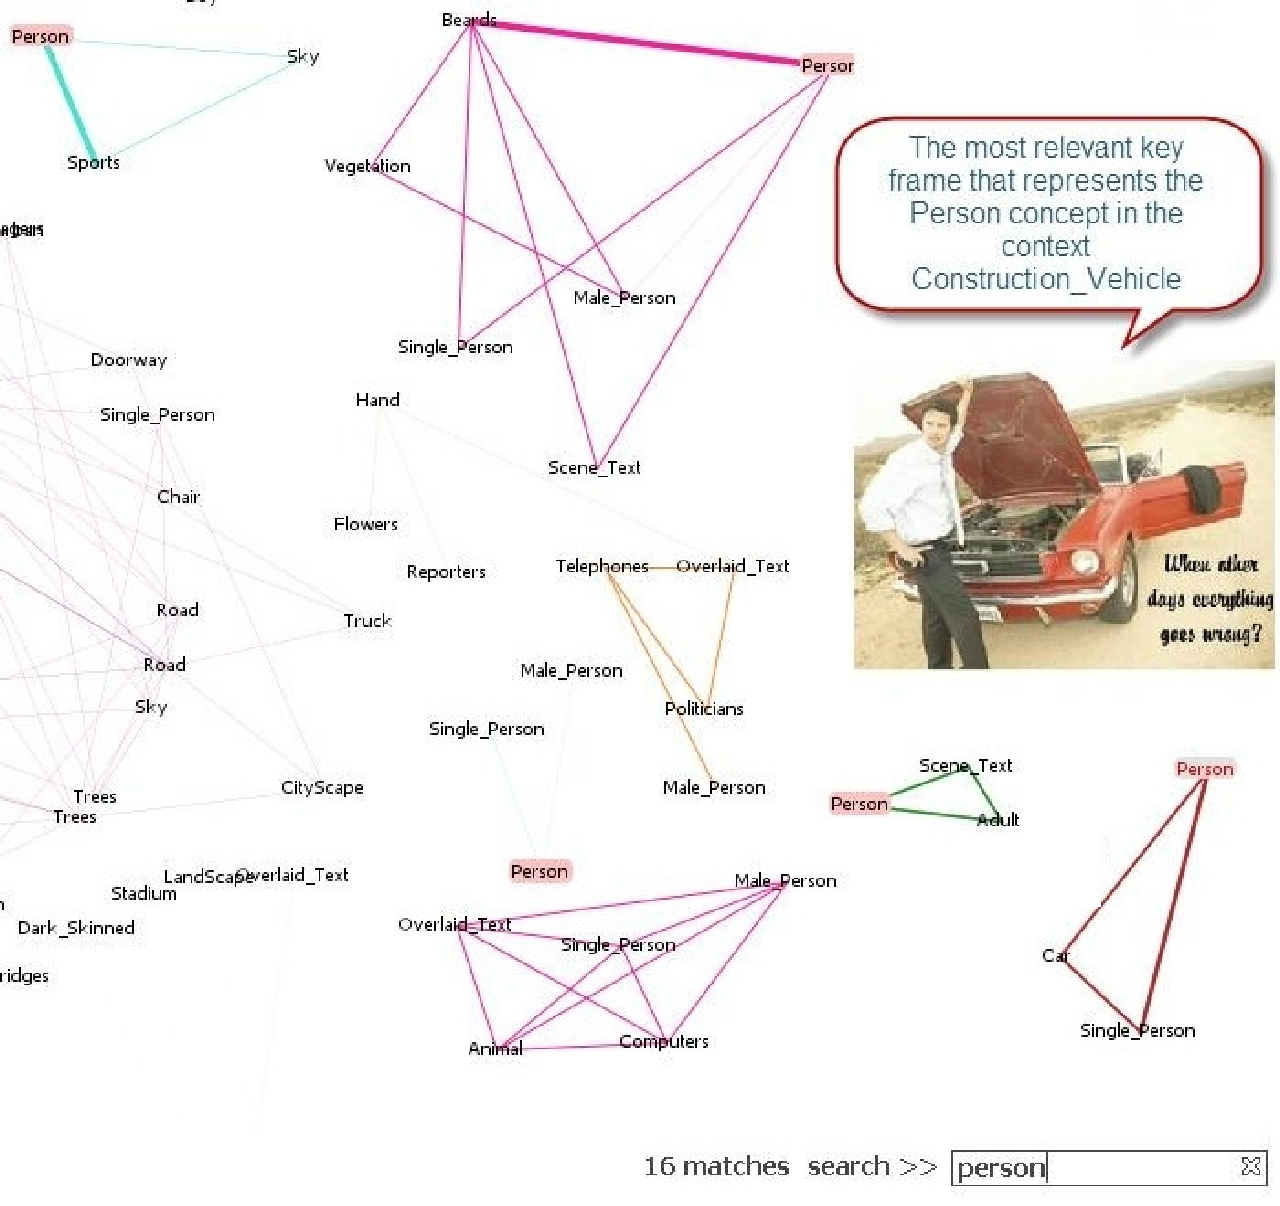
\includegraphics[scale=0.3]{graphics/vis}
			\caption{Visualization of conceptual relationships}
			\label{fig4444}
		\end{figure}


\begin{figure}[ht!]	
			\centering
			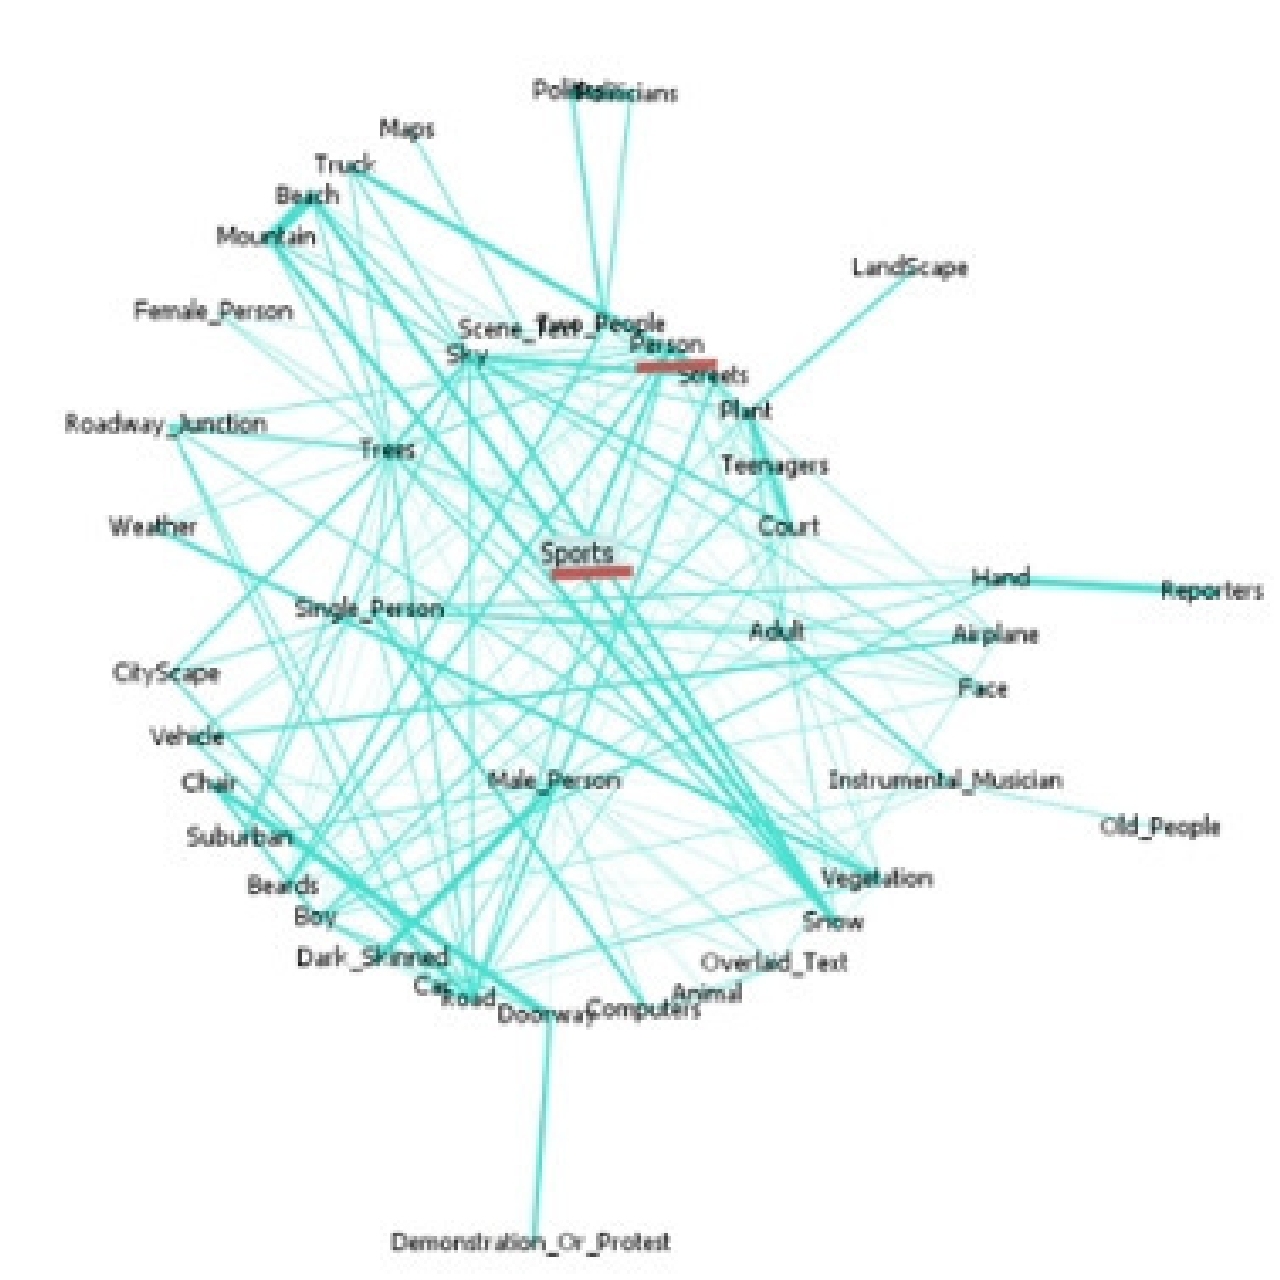
\includegraphics[scale=0.3]{graphics/figa}
			\caption{Conceptual relationships graph without contextual notion}
			\label{figa}
		\end{figure}

\section{Assessment}

In order to assess the performance of our proposed annotation tool, we conduct an experimentation. The aim of such assessment is to check the effectiveness of our proposed annotation tool.

To evaluate our approach within a real examples, we used a set of video sequences from available \textsc{TrecVid} video dataset.  Ten users (annotators) annotated about one hour of video.
We defined so 120 concepts and 29 contexts to be annotated. We show, in what follows, the contribution of integration of contextual notion in the annotation process.

	\subsection{Conceptual relationships without contextual information}

The figure \ref{figa}  illustrates the relationships computed by analyzing inter-concept similarities (without taking into consideration the context space). In such situation,  and for two given concepts, we obtain only one similarity value. For example, the concepts \textit{Person} and \textit{Sports}, are similar with a value of $0.39$.

		

	\subsection{Conceptual relationships incorporating contextual information}

Since a concept could have different meaning according to the context in which it exists, it is obvious to take into consideration that context when computing similarity for defining conceptual relationships. Therefore, the figure \ref{fig4444} displays two sub-graphs. Each sub-graph presents the semantic relationships according to a given context.

As an example, the relationships between the two concepts \textit{Sports} and \textit{Person} is different according to the defined context. In the context \textit{ Outdoor}, the relationships is valued by $0.055$. But in the context \textit{ Walking-Running}, that relationship is valued by $0.7$.

We can conclude that the context \textit{ Walking-Running} highlight better the relationship between the two concepts \textit{Sports} and \textit{Person}. 
		


	\subsection{Correlation between the frequency of concept and the annotators disagreement}
\begin{figure}[ht!]	
			\centering
			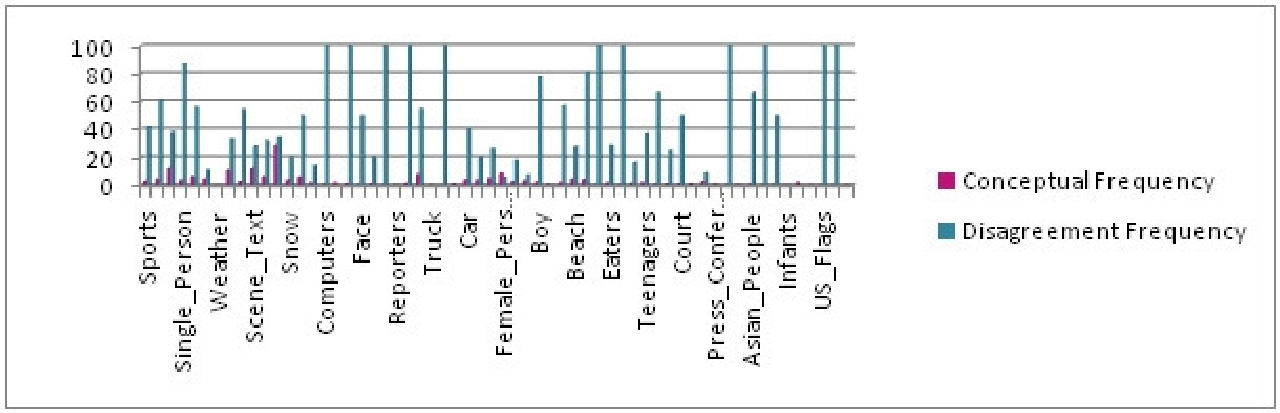
\includegraphics[scale=0.3]{graphics/figb}
			\caption{Correlation between concept frequency and annotators disagreement}
			\label{figb}
		\end{figure}
		\begin{figure}[ht!]	
			\centering
			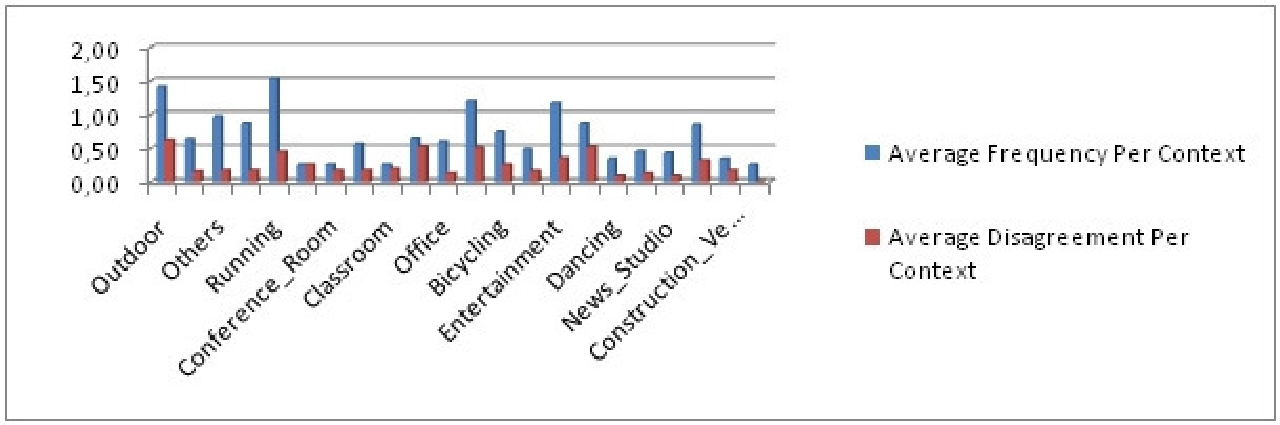
\includegraphics[scale=0.3]{graphics/figc}
			\caption{Correlation between concept average frequency and annotators average disagreement}
			\label{figc}
		\end{figure}
In figure \ref{figb}, we notice a strong relationship between concept frequency and the rate of  disagreement of inter-annotators for each concept. In our case, we define a  disagreement as a case where at least one annotator indicates that a concept does not exist in a photo when the other annotators indicates that this concept exists. 

More concepts are annotated, more the disagreement rate decreases. This correlation  displays the performance of our annotation tool in which we try to avoid such a situation by integrating the collaborative aspect and particularly the sharing of preceding annotations.

Figure \ref{figc} presents the concepts average  frequency and the average disagreement in each detected context. We conclude that the concepts in the contexts \textit{Airplane-Flying}, \textit{Bicycling}, and \textit{Running} are clear to identify them with a reduced disagreement rate.

\section{Conclusion}

The present chapter introduce a novel tool for collaborative video annotation. The proposed system provides a simple interface that includes a set of assistance tools such as graphical concept relationships visualization which allows the annotator to easily interpret data and annotate a video content. Our annotation tool does not handle conflicts but tries to avoid it by integrating the collaborative aspect and sharing previous annotations. 
One interesting aspect of our approach is the use of a contextual graph which is generated during and after the annotation process. This graph is very useful for giving more meaning to the annotated data, indexing systems and for information retrieval systems and specifically in query mapping.



		


